\documentclass{article}
\usepackage{import}
\usepackage[ruled]{algorithm2e}
\usepackage[shortlabels]{enumitem}
\usepackage{hyperref}
\usepackage{minted}
\usepackage{subcaption}
\hypersetup{
    colorlinks=true,
    linkcolor=blue,
    filecolor=magenta,      
    urlcolor=cyan,
    pdftitle={Overleaf Example},
    pdfpagemode=FullScreen,
    }
\subimport*{}{macro}

\setlength\parindent{0px}

\begin{document}
\setcounter{problem}{0}
\title{Homework \#5}
\author{
    \normalsize{AA 597: Networked Dynamics Systems}\\
    \normalsize{Prof. Mehran Mesbahi}\\
    \normalsize{Due: Feb 16, 2024 11:59pm}\\
    \normalsize{Soowhan Yi}
}
\date{{}}
\maketitle

All the codes are available at the end of the documents or here.
\url{https://github.com/SoowhanYi94/ME597}
\begin{problem}7.1
    This chapter mainly dealt with $\Delta$-disk graphs, that is, proximity graph (V,E) such that ${v_i, v_j} \in E$ if and only if $||x_i - x_j|| \leq \Delta$. wjere $x_i \in R^p, i = 1, \cdots, n, $ is the state of robot i. In this exercise, we will be exploring another type of proximity graphy, namely the wedge graph. Assume that instead of single integrator dynamics, the agents' dynamics are defined as unicycle robots, that is, 
    \begin{align*}
        &\dot x_i(t) = v_i(t) cos{\phi_i (t)}\\
        &\dot y_i(t) = v_i(t) sin{\phi_i (t)}\\
        &\dot \phi_i(t)= \omega_i(t)
    \end{align*}
    
    Here $[x_i, y_i]^T$ is the position of robot i, while, $\phi_i$ denotes its orientation. Moreover, $v_i$ and $\omega_i$ are the translational and rotational velocities, which are the controlled inputs. Now, assume that such a robot is equiopped with a rigidly mounted camer, facing in the forward direction. This gives rise to a directed wedge graph, as seen in the figure. For such a setup, if robot j is visible from robot i, the available information is $d_{ij} = ||[x_i, y_i]^T - [x_j, y_j]^T||$ (distance between agents) and $\delta \phi_{ij}$(relative interagent angle) as per the figure below. Explain how you would solve the rendezvous (agreement) problem for such a system. 
    
    \vspace{12pt}
    In order to solve this agreement problem, we need to controll the distance between two agents, especially between the leaf nodes($v_j$ and $v_k$ in the example) and the center node($v_i$), and angle between them. We have a sector form of sensing area, and we need to keep them inside in order to stay connected. So we construct a potential function of $V_i = \sum_{j \in N(i) }(\frac{1}{(\delta \phi_{ij} - \frac{\Delta \psi}{2})^2} + \frac{d_{ij}^2}{\rho - d_{ij}})$. Then, 
    \begin{align*}
        v_i(t)&=\dot r_i(t) = \sum_{j \in N(i) }-\frac{dV_{i}}{d (d_{ij})}= -\sum_{j \in N(i) }\frac{2\rho  - ||d_{ij}||}{(\rho  - ||d_{ij} ||)^2} (r_{i} - r_{j} ) \\
        \dot x_i(t) &= -\sum_{j \in N(i) }\frac{2\rho  - ||d_{ij}||}{(\rho  - ||d_{ij} ||)^2} (r_{i} - r_{j} ) \cos(\delta \phi_{ij})\\
        \dot y_i(t) &= -\sum_{j \in N(i) }\frac{2\rho  - ||d_{ij}||}{(\rho  - ||d_{ij} ||)^2} (r_{i} - r_{j} ) \sin(\delta \phi_{ij})
    \end{align*}
    where this i corresponds to those robot agents. From lemma 7.1 from textbook proves that $\Omega (\rho, r_0) = \curly{r| V(\rho, r) \leq V(\rho, r_0)}$ is invariant set under the above control law, where $r_0 \in D_{G, \rho} ^\epsilon$ for $\epsilon \in (0, \rho)$. Also the theorem 7.2 from textbook proves that this control law asymptotically converges to the static centroid. 

    Now we need to keep the angles between them to be in certain range, and I would use the same logic that was used in above equation.
    \begin{align*}
        \omega_i = \dot {\delta \phi_{ij}}(t) &= - \sum_{j \in N(i) }\frac{-2}{( \delta \phi_{ij}-\frac{\Delta \psi}{2})^3} 
    \end{align*}
    With above equations, agents are guranteed to stay in the sector shaped sensing area. Since we have $\delta \phi_{ij}^0 \leq \frac{\Delta \psi}{2}$, this $\delta \phi_{ij}(t)$ would never increase. Therefore angle between them would never increase and distance would converge to their static centroid. 


\end{problem}
\begin{problem}
Show that if a $\delta$-disk proximity graph with 4 agents starts connected, then, using the linear agreement protocol, it stays connected for all times.

With theorem 3.4  in the textbook, we know that the linear agreement protocol converges to the agreement set. Therefore the length of edges between two vertices would never increase. Even with the case where 2 nodes (node 1 and node 2)are located in one points $\Delta$ away from node 3, and node 4 is located $\Delta$ away from node 3 and $2 \Delta$ away from node 1 and 2, we proved that they do converge in one point with 4 agents from last homework(4.8). As we have started with each lengths of edges being less than or equal to $\Delta$, those lengths would stay less than $\Delta$ in the progress of the linear agreement protocol and until it reaches the agreement. 


\end{problem}
\begin{problem}
    \begin{align*}
        \dot x_i(t) &= -\sum_{j \in N_{G_d}(i)} \frac{2(\Delta - ||d_{ij}||) - ||l_{ij} - d_{ij}||}{(\Delta - ||d_{ij}|| - ||l_{ij} - d_{ij}||)^2} (x_i(t) - x_j(t) - d_{ij} )
    \end{align*}
    Lemma 7.5\\
    Given an initial conditions $x_0$ such that $y_0 = (x_0 - \tau_0) \in D_{G_{d}, \Delta -||d||}^\epsilon$, with $G_d$ a connected spanning graph of $G(x_0)$, the group of autonomous mobile agents adopting the decentralized contral law (the equation above) are guranteed to satisfy
    \begin{align*}
        ||x_i(t) - x_j(t)|| = ||l_{ij}(t)|| \leq \Delta \text{ for all } t > 0 \text{ and }{ v_i, v_j} \in E_d
    \end{align*}

    Theorem 7.6
    Under the same assumptions as in Lemma 7.5, for all i, j, the pairwize relative distants $||l_{ij}|| = ||x_i(t) - x_j(t)||$ asymptotically converge to $||d_{ij}||$ for ${v_i, v_j} \in E_d$
    
    \vspace{12pt}
    Implement the algorithm above and explore how the conditions of Lemma 7.5/Thm 7.6 are required for the algorithm to work as proposed.
    \begin{figure*}[!h]
        \centering
        \begin{subfigure}{0.3\textwidth}
            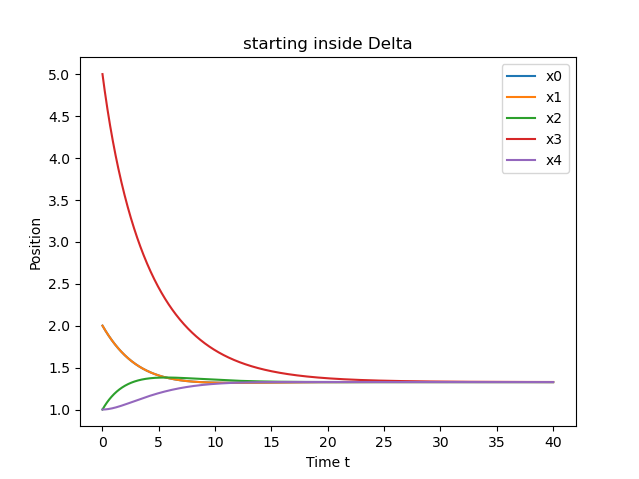
\includegraphics[width=\textwidth]{./img/p3_1.png}
            \caption{$||x_i - x_j|| \leq \Delta$}
        \end{subfigure}
        \begin{subfigure}{0.3\textwidth}
            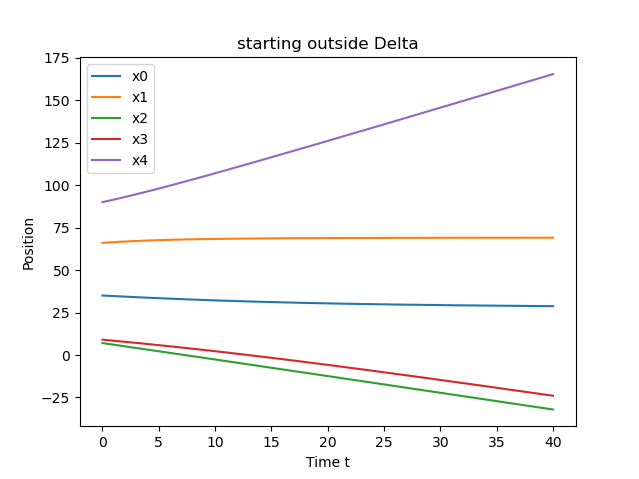
\includegraphics[width=\textwidth]{./img/p3_2.png}
            \caption{$||x_i - x_j|| \nleq \Delta$}
        \end{subfigure}
        \begin{subfigure}{0.3\textwidth}
            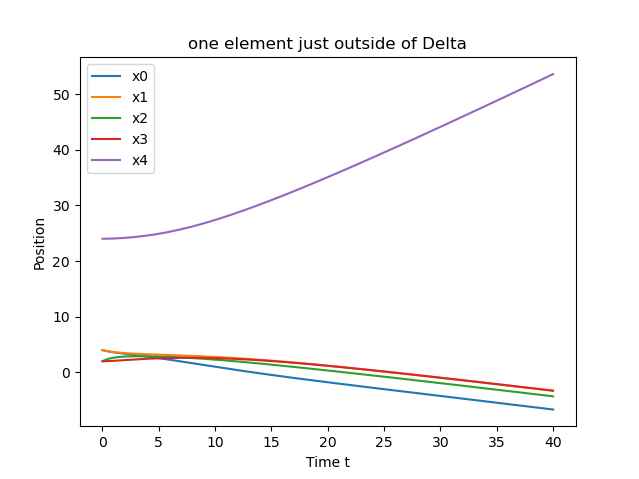
\includegraphics[width=\textwidth]{./img/p3_3.png}
            \caption{$||x_4 - x_j|| \nleq \Delta$ }
        \end{subfigure}
    \end{figure*}

    For above graphs, the desired lengths between each nodes are set to be 0 for simplicity. As we can see from above results, when those initial conditions satisfy those conditions of Lemma 7.5 and theorem 7.6, above algorithm asymptotically converges to edge length of 0. Also, those that are not satisfing those conditions ($x_0, x_3, x_4$ in (b), and $x_4$ in (c)) are diverging and those that are satisfing conditions ($x_1, x_2$ in (b), and $x_0, x_1, x_2, x_3$ in(c)) are converging. Also, when $||x_i - x_j|| = \Delta$, above algorithm does not compute because we would be getting infinite number when the desired length for edges are 0. So we need this threshold $\epsilon$ for computation. Therefore this algorithm, in order to work properly, those conditions of Lemma 7.5 and theorem 7.6 are required. 
\end{problem}

\begin{problem}
    11.2 Show that if $\lambda_2(G)$ has an algebraic muliplicity m in in the graph G, then adding up to m edges will not improve it. 

\end{problem}
\begin{problem}
    11.10 Use the approach of section11.6 and a semidefinite programming
    solver (such as the one mentioned in notes and references), to maximize
    $\lambda_2 (G)$ for the weighted versions of K5 , P5 , and S5 , subject to a normalization on the sum of the weights. Comment on any observed patterns for the
    optimal weight distribution.
\end{problem}
\newpage
\section*{Code}
\begin{minted}{python3}
\end{minted}
\end{document}